\chapter{Meal Forecasting}
\label{meal-forecasting}

Based on the historical data of meal purchases aggregated by week, spanning 145 weeks for each center, the initial objective of this project is to forecast the quantity of each food item that every distribution center will require. This prediction will involve analyzing the demand trends for each food item across the different centers, and identifying any patterns or seasonality in the data. The accurate forecasting of meal orders for each center will enable the company to efficiently plan and allocate resources, ensuring that they can meet the anticipated demand and minimize waste.

\section{Details}
\label{meal-forecasting-details}
The first reference metric is to take the average of N previous weeks and project it into the future, this is both easy to implement and quite accurate.

The second approach involves utilizing the widely used library, Prophet~\cite{taylor2018forecasting}, to capture the seasonality and trends in the demand data and project them into the future. In order to simplify the problem, we did not consider other additional data such as pricing, product features, or promotions. Instead, we solely focused on the number of orders per week. While this simplified approach negatively impacted the performance and precision of the model, we decided that it was the best option given the project's time constraints.

Given the high quantity of meal-facility pairs to analyze, the project also implements a multi-processing optimization that splits the computation load across the present CPU cores.

\section{Results}
\label{meal-forecasting-results}
To compare the results we will divide the data between training and testing, after that we compare the Mean Square Error of the whole dataset for the various strategies. To offer a better interpretation, 9 randomly selected meal-facility pairs have been plotted.

The only hyper-parameter involved in the first strategy is the number of weeks to average the demand data. After conducting several manual trials, we optimized this parameter to three weeks.


\begin{figure}[tb]
    \centering
    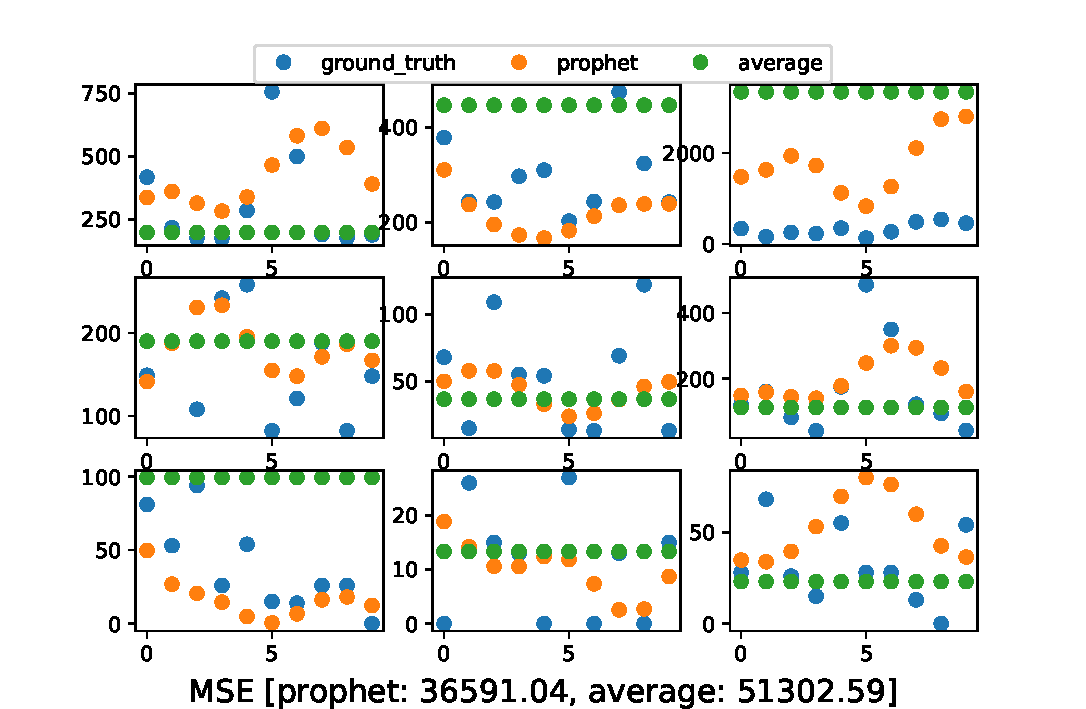
\includegraphics[width=1\columnwidth]{figures/meal_forecast_res_long.pdf}
    \caption{Meal Forecast results, 10 weeks}
  \label{fig:meal-forecast-res-long}
\end{figure}

As demonstrated in Figure~\ref{fig:meal-forecast-res-long}, the Prophet forecasting strategy outperforms the simple average approach in terms of accuracy, even without the use of auxiliary data. The Prophet model is able to capture the underlying trends and patterns in the demand data more effectively, and provide more accurate forecasts for future weeks. However, this advantage is not as significant when it comes to single-week forecasting.

\begin{figure}[tb]
    \centering
    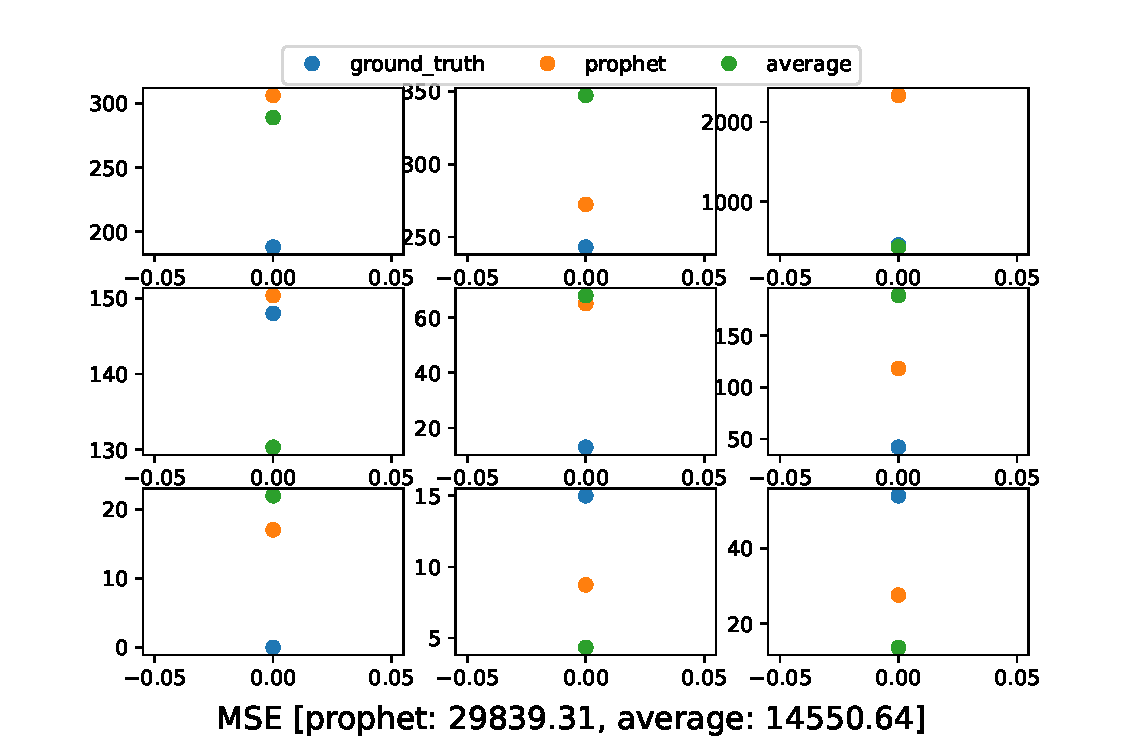
\includegraphics[width=1\columnwidth]{figures/meal_forecast_res_short.pdf}
    \caption{Meal Forecast results, 1 week}
  \label{fig:meal-forecast-res-short}
\end{figure}

However, as depicted in Figure~\ref{fig:meal-forecast-res-short}, when forecasting the outcome for a single week in advance, the average solution appears to provide better results. Although this could be attributed to inadequate utilization of the library or the presence of data outliers, we opted to proceed with the data that produced lower error since that part falls out of the project scope.
